% !TEX root = EUDAQUserManual.tex
\section{Integration with User Hardware}\label{sec:Integration}
EUDAQ itself is only a data taking framework which provides the common feature. It means that the users with their dedicated hardware and readout software are required to write some code to bridge the hardware specific readout software to EUDAQ frame work. The minimum adaption task is to have write a Producer for each piece of hardware, a Data Collector to receive the data (aka. Event) from Producers. 

\subsection{Announcement of Derived Class}
The derived EUDAQ classes provided user will compiled and packed to a dynamic shared library (EUDAQ Module Library). At compiling/linking time of EUDAQ core library, it does not know the existing of any Module Library. When EUDAQ core library is been loading by any application, the core library will looking any library file with name prefix libeudaq\_module\_ in the module folder. All pattern matched library are going to be loaded. It is the time point when each derived EUDAQ class announces itself to the EUDAQ runtime environment.

Technically, the announcement of a derived class is done by a calling to the correlated static function provided by a generic C++ template (eudaq::Factory). Tab. \autoref{tab:derivable} is the list of derivable EUDAQ classes

\begin{table}
\centering
\small
\begin{tabular}{ l | l }
  \textbf{Class} & \textbf{Description}\\
  \hline
  \texttt{eudaq::Producer} & Sec. \ref{sec:ProducerWriting}\\
  \texttt{eudaq::DataCollector} & Sec. \ref{sec:DataCollectorWriting}\\
  \texttt{eudaq::RunControl} & Sec. \ref{sec:RunControlWriting}\\
  \texttt{eudaq::Event} &  \\
  \texttt{eudaq::LogCollector} & \\
  \texttt{eudaq::Monitor} & Sec. \ref{sec:MonitorWriting}\\
  \texttt{eudaq::FileWriter} & Sec. \ref{sec:FileWriterWriting}\\
  \texttt{eudaq::FileReader} & Sec. \ref{sec:FileReaderWriting}\\
  \texttt{eudaq::StdEventConverter} & \\
  \texttt{eudaq::LCEventConverter} & \\
  \texttt{eudaq::TransportServer} & internal only \\
  \texttt{eudaq::TransportClient} & internal only \\
\end{tabular}
\caption{Derivable Classes.}
\label{tab:derivable}
\end{table}

\subsection{Serializable}
As a distributed DAQ framework, a runtime setup of EUDAQ system include several applications. Data objects will go through the boundary of an application or a computer. Those data objects should have the capability to be serialized. When a data object is serialized, all the crucial data of this data object is feed to serialized memory which then can be send by plain binary to another application and reconstructed to a copy of original data object. \\

All the classes which hold serializable data are derived from a base serializable class (eudaq::Serializable). All serializable data class
should implement the function \texttt{Serialize} which serializes the inner data object and feeds a eudaq::Serializer, and a constructor function which takes the reference of eudaq::Deserializer as input parameter.\\

\autoref{tab:serializable} is the list of serializable EUDAQ classes.

\begin{table}
\centering
\small
\begin{tabular}{ l | l }
  \textbf{Class} & \textbf{Description}\\
  \hline
  \texttt{eudaq::Event} & \\
  \texttt{eudaq::Configuration} & \\
  \texttt{eudaq::LogMessage} & \\
  \texttt{eudaq::Status} &  \\
\end{tabular}
\caption{Serializable Classes.}
\label{tab:serializable}
\end{table}

\subsubsection{Event}
eudaq::Event is most important serializable class which holds physics data from hardware. Producer is the EUDAQ component which create object of eudaq::Event and feed it by the physics data from measurement.  \autoref{tab:serializable} lists the variables inside the eudaq::Event. \\

\begin{table}
\centering
\small
\begin{tabular}{ l | l | l }
  \textbf{variable} & \textbf{C++ type} & \textbf{Description}\\
  \hline
  \texttt{m\_type} & \texttt{uint32\_t} & event type\\
  \texttt{m\_version} & \texttt{uint32\_t} & version\\
  \texttt{m\_flags} & \texttt{uint32\_t} & flags\\
  \texttt{m\_stm\_n} & \texttt{uint32\_t} & device/stream number\\
  \texttt{m\_run\_n} & \texttt{uint32\_t} & run number\\
  \texttt{m\_ev\_n} & \texttt{uint32\_t} & event number\\
  \texttt{m\_tg\_n} & \texttt{uint32\_t} & trigger number\\
  \texttt{m\_extend} & \texttt{uint32\_t} & reserved word\\
  \texttt{m\_ts\_begin} & \texttt{uint64\_t} & timestamp at the begin of event\\
  \texttt{m\_ts\_end} & \texttt{uint64\_t} & timestamp at the end of event\\
  \texttt{m\_dspt} & \texttt{std::string} & description\\
  \texttt{m\_tags} & \texttt{std::map<std::string, std::string>} & tags\\
  \texttt{m\_blocks} & \texttt{std::map<uint32\_t, std::vector<uint8\_t>>} & blocks of raw data\\
  \texttt{m\_sub\_events} & \texttt{std::vector<EventSPC>} & pointers of sub events\\
\end{tabular}
\caption{Variables of eudaq::Event.}
\label{tab:eventdata}
\end{table}

The \texttt{m\_blocks} is physics data which only can be known by the user who owns the hardware. There is a pair of timestamps to define the time slice when the physics event occurs, and a trigger number to identify the trigger sequence. Timestamps and trigger number are optional to be set if you are going to use them to synchronize data from multiple stream/device. It is also possible to have sub events inside an eudaq::Event object. The sub eudaq::Event objects is hold by std::shared\_ptr. See next sub section.

\subsection{Ownership}
std::shared\_ptr and std::shared\_ptr is heavily used in EUDAQ to hold the object pointer of serializable class and derivable class. It gets rid of the unnecessary and ineffective memory copy and is exception safe for any memory leaking.

\subsection{Command/Status Handling}
\subsubsection{RunControl and CommandReceiver}\label{sec:fsm}
\paragraph{RunControl} eudaq::RunControl is the command sender which issue command according to user actions from GUI or CLI.
\paragraph{CommandReceiver} eudaq::Producer, eudaq::DataCollector, eudaq::LogCollector and eudaq::Monitor are command receivers (eudaq::CommandReceiver) which executes the correlated function according the command. The command receiver will set up a status (eudaq::Status) and report the status to RunControl.

\subsubsection{State Model}\label{sec:fsm}
\begin{figure}
\begin{center}
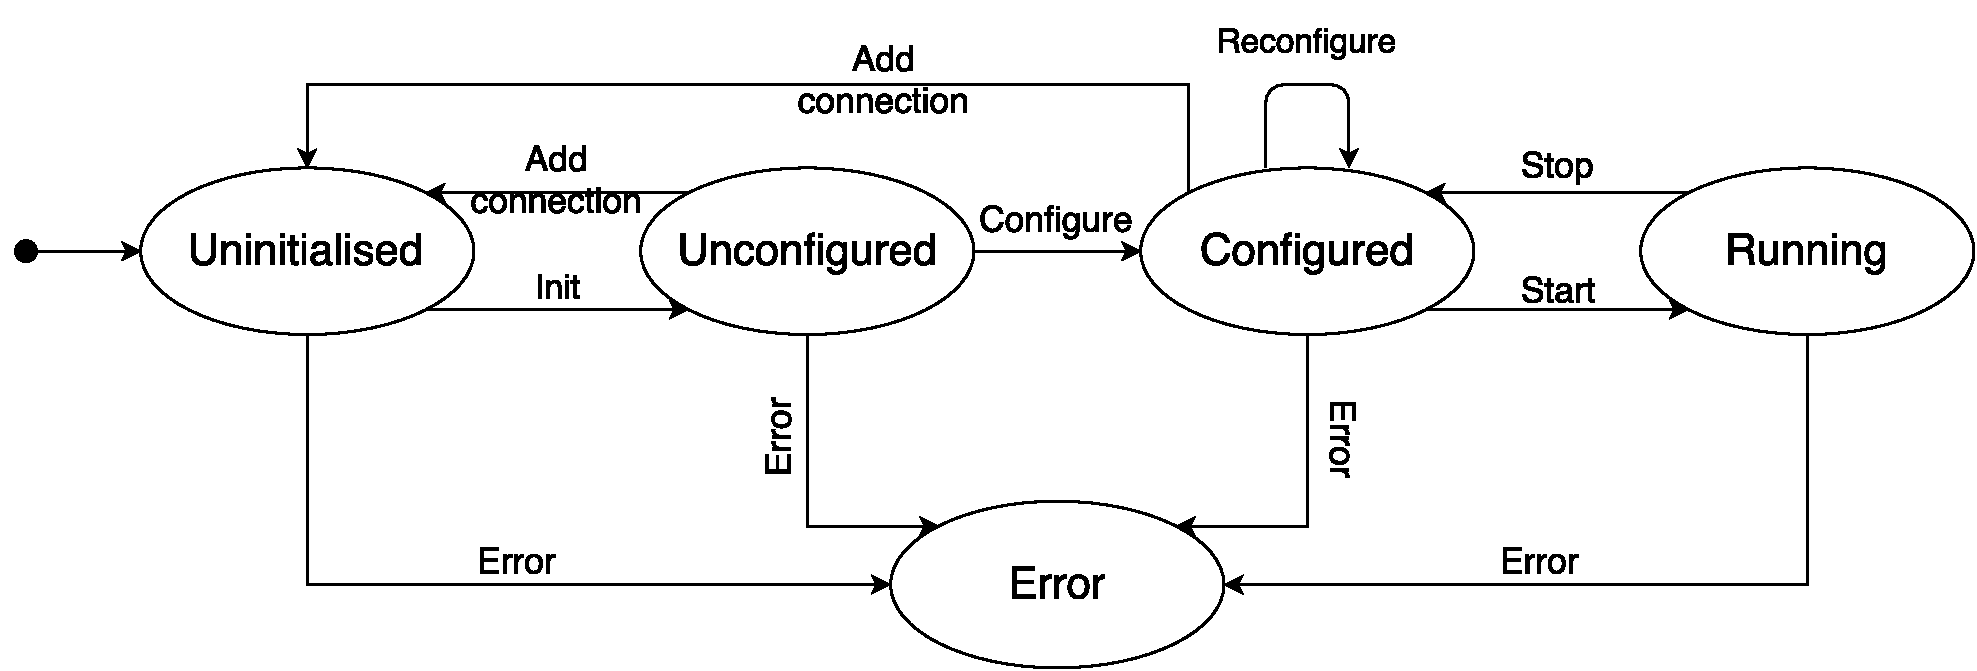
\includegraphics[width=0.9\textwidth]{src/images/fsmv2.pdf}
\end{center}
\caption{The FSM of EUDAQ.}
\label{fig:fsm}
\end{figure}

The finite-state machine \gls{FSM} is implemented to both RunControl and CommandReceiver (see \autoref{fig:fsm}) \cite{Shirokova:2016}. \\

Each command receiver can always be characterized by the current state (\autoref{tab:statetab})
\begin{table}
\centering
\small
\begin{tabular}{ l | l | l | l }
  \textbf{State} & \textbf{Enumerate Value} & \textbf{Acceptable Command} & \textbf{Description}\\
  \hline
  \texttt{Error} & \texttt{eudaq::Status::STATE\_ERROR} & DoReset & \\
  \texttt{Uninitialised} & \texttt{eudaq::Status::STATE\_UNINIT} & DoInitialise DoReset & the initial state of every client. Initialization has not been conducted\\
  \texttt{Unconfigured} & \texttt{eudaq::Status::STATE\_UNCONF} & DoConfigure DoReset & \\
  \texttt{Configured} & \texttt{eudaq::Status::STATE\_CONF} & DoConfigure DoStartRun DoReset & \\
  \texttt{Running} & \texttt{eudaq::Status::STATE\_RUNNING} & DoStopRun & \\
\end{tabular}
\caption{States of RunControl client}
\label{tab:statetab}
\end{table}


The state of RunControl is determined by the lowest state of the connected client in the following priority: ERROR, UNINITIALISED, UNCONFIGURED, CONFIGURED, RUNNING. It means, for example, that even if only one connection is in the ERROR state, the whole machine will also be in that state. This prevents such mistakes as running the system before every component has finished the configuration.

\subsubsection{Command}\label{sec:command}

\begin{table}
\centering
\small
\begin{tabular}{ l | l | l | l |l }
  \textbf{Command} & \textbf{RunControl Side} & \textbf{Client Side} & \textbf{Pre State} & \textbf{State of Success}\\
  \hline
  \texttt{Initialise} & Initialise & DoInitialise & Uninitialised & Unconfigured\\
  \texttt{Configure} & Configure & DoConfigure & Unconfigured Configured & Configured\\
  \texttt{StartRun} & StartRun & DoStartRun & Configured & Running\\
  \texttt{StopRun} & StopRun & DoStopRun & Running & Configured\\
  \texttt{Reset} & Reset & DoReset & Error & Uninitialised\\
\end{tabular}
\caption{List of Commands}
\label{tab:cmdtab}
\end{table}


\paragraph{Initialise}
When an EUDAQ process is on the state of Uninitialised, it accepts Initialise command and execute the DoInitialise function provided by user. When it is initialized, it does not accept further Uninitialised command any more until it is reseted to Uninitialised state.

\paragraph{Configure}
When an EUDAQ process is on the state of Unconfigured or Configured, it accepts Configure command and execute the DoConfigure function provided by user. Please be aware that the second Configure command after a successful execution of Configure command is allowed. It means EUDAQ process is re-configurable but not re-initialisible.

\paragraph{StartRun}
When an EUDAQ process is on the state of Configured, it also accepts StartRun command and execute the DoStartRun function provided by user. In case of Producer, the Producer should talk to the underline hardware and produce and send Event data. In case of DataCollector, the DataCollector will get the Event stream from its connected Producer.

\paragraph{StopRun}
When an EUDAQ process is on the state of Running, it only accepts StopRun command and execute the DoStopRun function provided by user. RunControl will not send the StopRun command to DataCollector until all Producers have returned from DoStopRun function and feedback their status.

\paragraph{Reset}
In any case when an EUDAQ process goes to the state of Error, only Reset command is allowed.

\paragraph{Terminate}
Except for the state of Running, the terminate command is allowed on all other state. When the Terminate command is called, the EUDAQ process are going to be closed. If user has to do something before the exiting of EUDAQ process, DoTerminate function is correct position to do the exiting route.

